% !TeX root = master.tex
% !TeX spellcheck = en_EN-EnglishUnitedKingdom

\appendix
\chapter{Appendix}
\label{sec:appendix}
\raggedbottom
\section{Supplementary Figures}
\subsection{Pairwise co-consumption}
\begin{figure}[H]
	\centering
	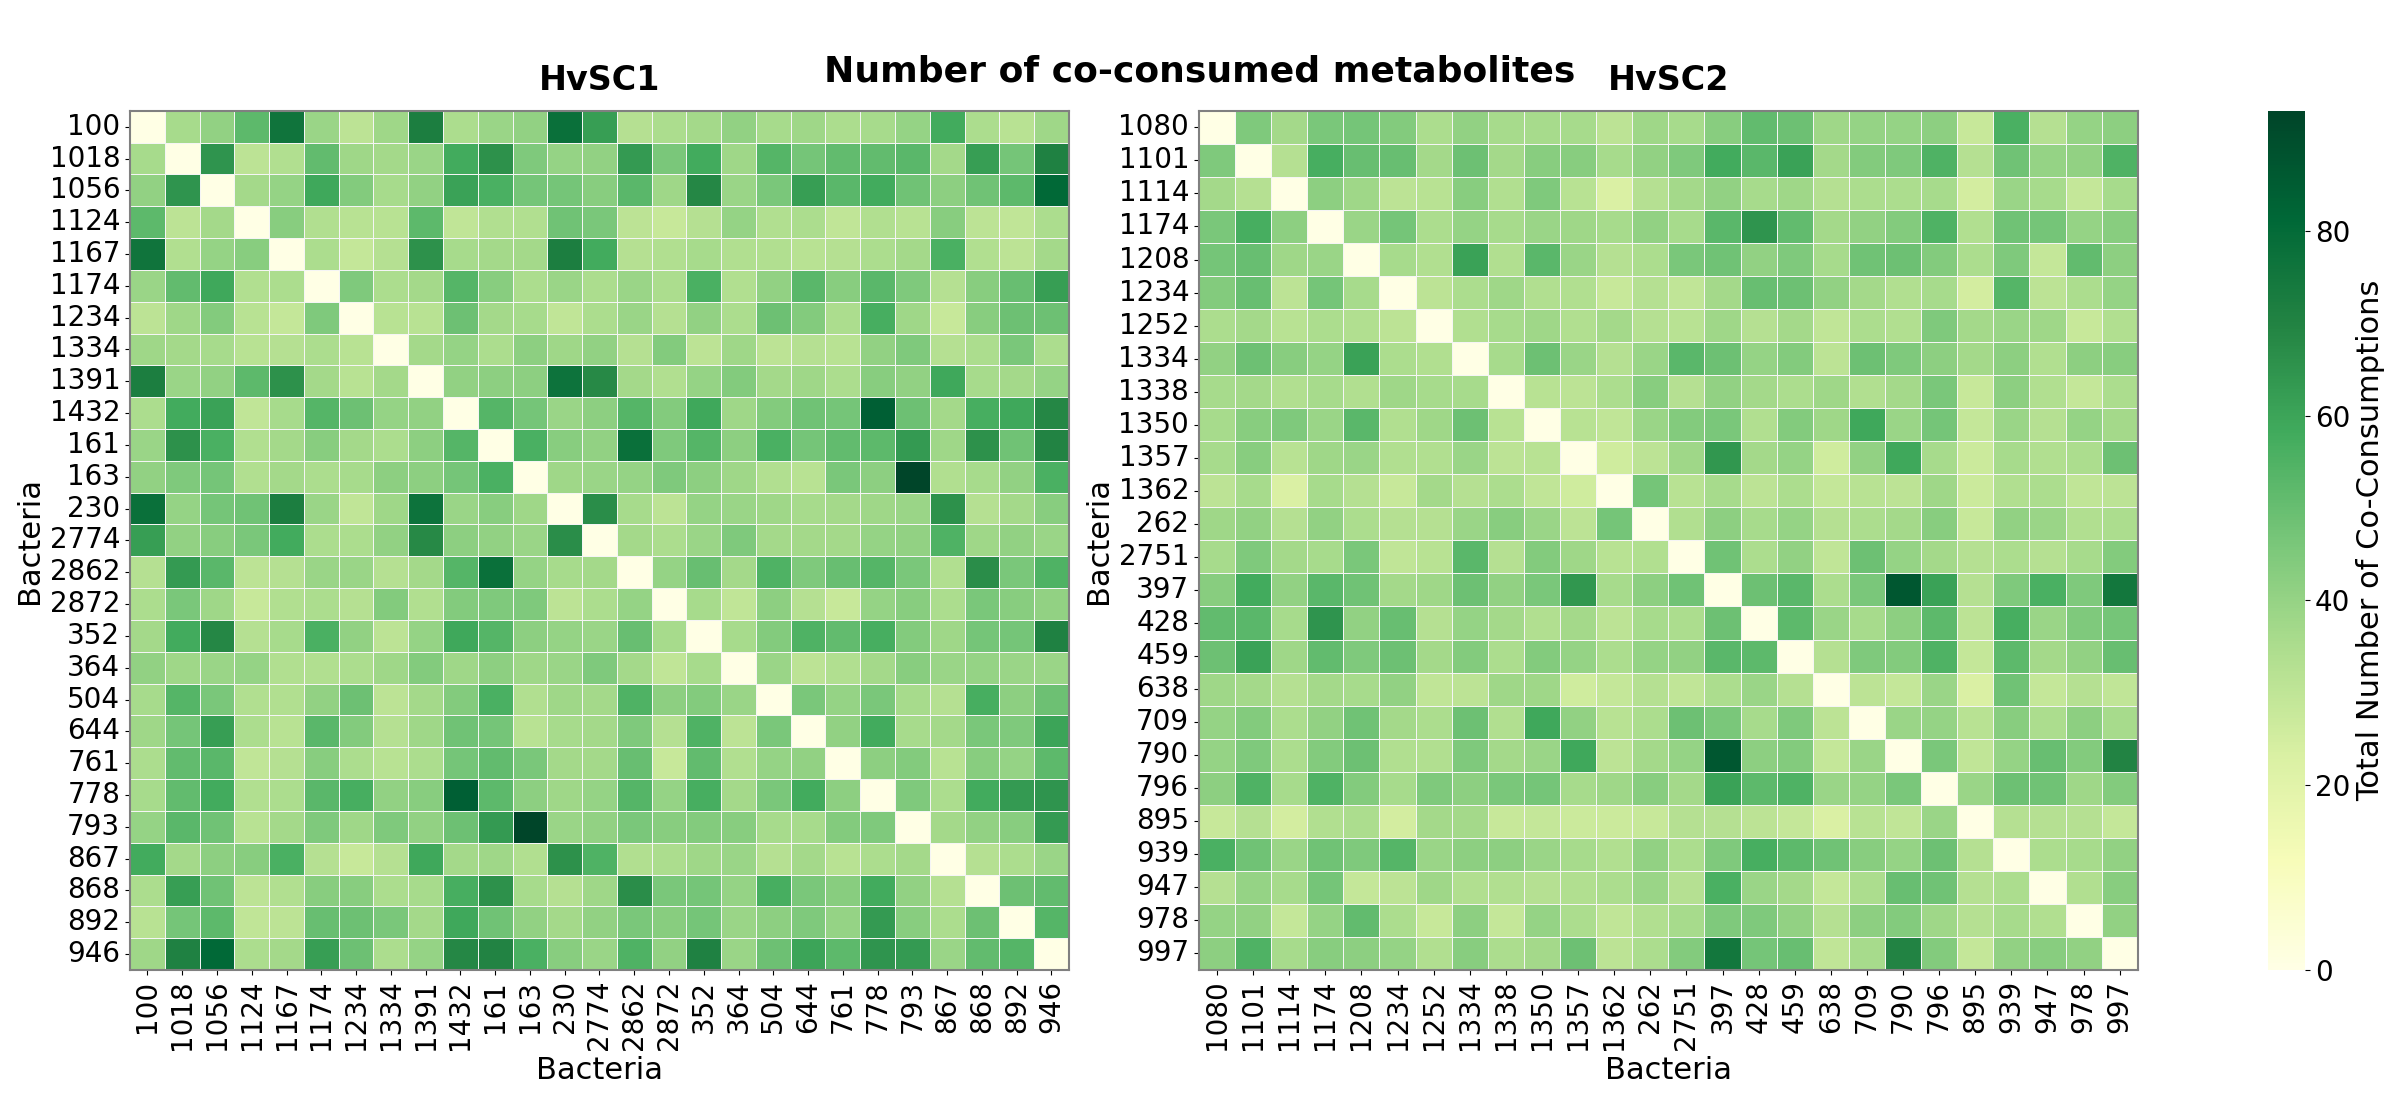
\includegraphics[width=1\linewidth]{fig/Combined_Numbercoconsumptions_heatmap}
	\caption[Number of pairwise co-consumptions]{Number of pairwise co-consumptions. Heatmaps show the total number of co-consumed metabolites for each pair of bacteria in HvSC1 (left) and HvSC2 (right). Rows and columns represent bacterial taxa, and darker green indicates a greater number of co-consumed metabolites. HvSC1 shows more co-consumed metabolites, compared to HvSC2.}
	\label{fig:combinednumbercoconsumptionsheatmap}
\end{figure}

\subsection{Medium generation process}

\begin{figure}[H]
	\centering
	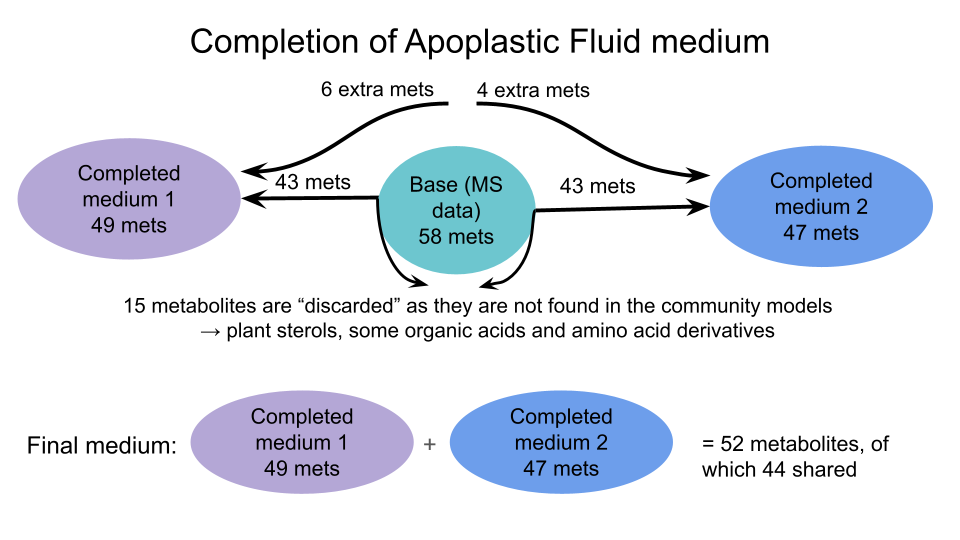
\includegraphics[width=1\linewidth]{fig/medium_completion_process}
	\caption[Medium completion process]{Completion of the apoplastic fluid medium. The base medium contained 58 metabolites derived from the MS data. After excluding 15 metabolites that were not detected in the community models, 43 metabolites were retained for each completed medium, with 6 additional metabolites added to medium 1 and 4 additional metabolites added to medium 2. The resulting media contained 49 and 47 metabolites, respectively. Combining both completed media yielded a final medium containing 52 unique metabolites, of which 44 were shared between the two communities.}
	\label{fig:medium_completion}
\end{figure}

\subsection{Impact of optimisation strategy on individual growth rates}

\begin{figure}[H]
	\centering
	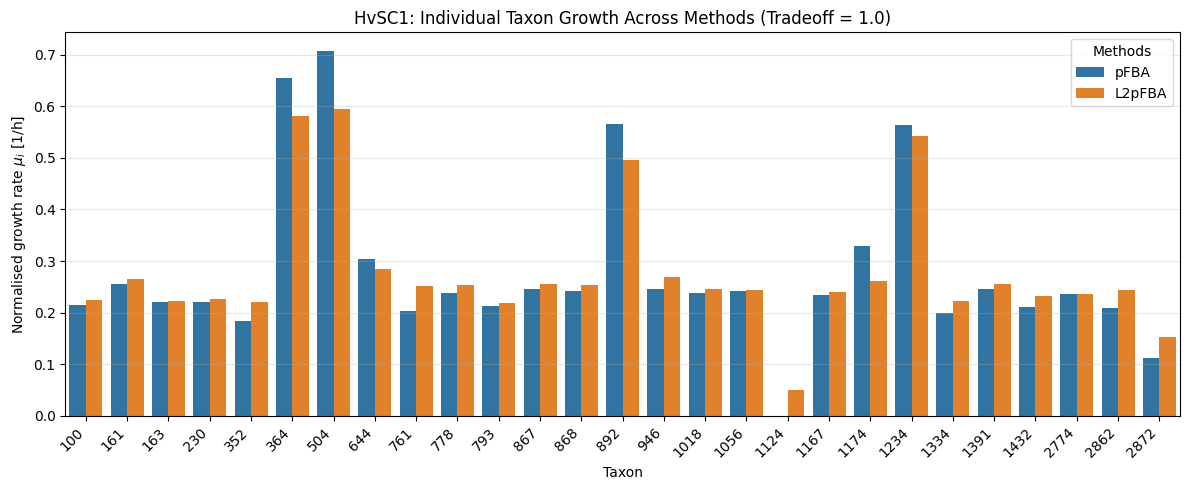
\includegraphics[width=1\linewidth]{fig/HvSC1_individual_growth_methods}
	\caption[Impact of optimisation strategy on individual growth rates of HvSC1]{Impact of optimisation strategy on individual growth rates of HvSC1. Barplot showing scaled $\mu_i$ of HvSC1 at trade-off $\alpha = 1.0$ for different optimisation strategies: pFBA only (blue) and L2-regularisation + pFBA (orange). L2-regularisation yields less extreme growth rates and ensures all strains grow.}
	\label{fig:hvsc1individualgrowthmethods}
\end{figure}

\begin{figure}[H]
	\centering
	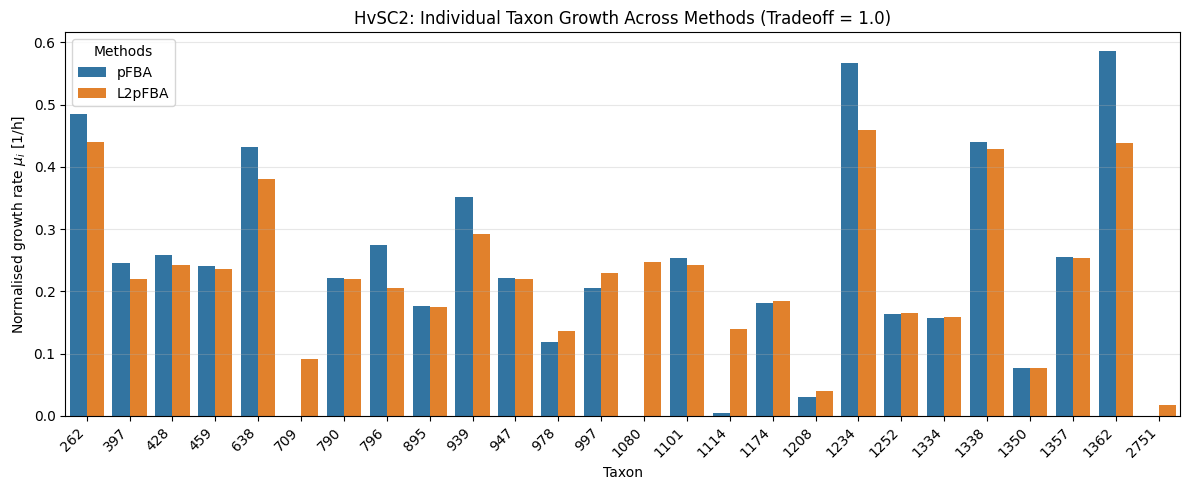
\includegraphics[width=1\linewidth]{fig/HvSC2_individual_growth_methods}
	\caption[Impact of optimisation strategy on individual growth rates of HvSC2]{Impact of optimisation strategy on individual growth rates of HvSC2. Barplot showing scaled $\mu_i$ of HvSC2 at trade-off $\alpha = 1.0$ for different optimisation strategies: pFBA only (blue) and L2-regularisation + pFBA (orange). L2-regularisation yields less extreme growth rates and ensures all strains grow.}
	\label{fig:hvsc2individualgrowthmethods}
\end{figure}


\subsection{Impact of trade-off value $\alpha$ on individual growth rates}
\begin{figure}[H]
	\centering
	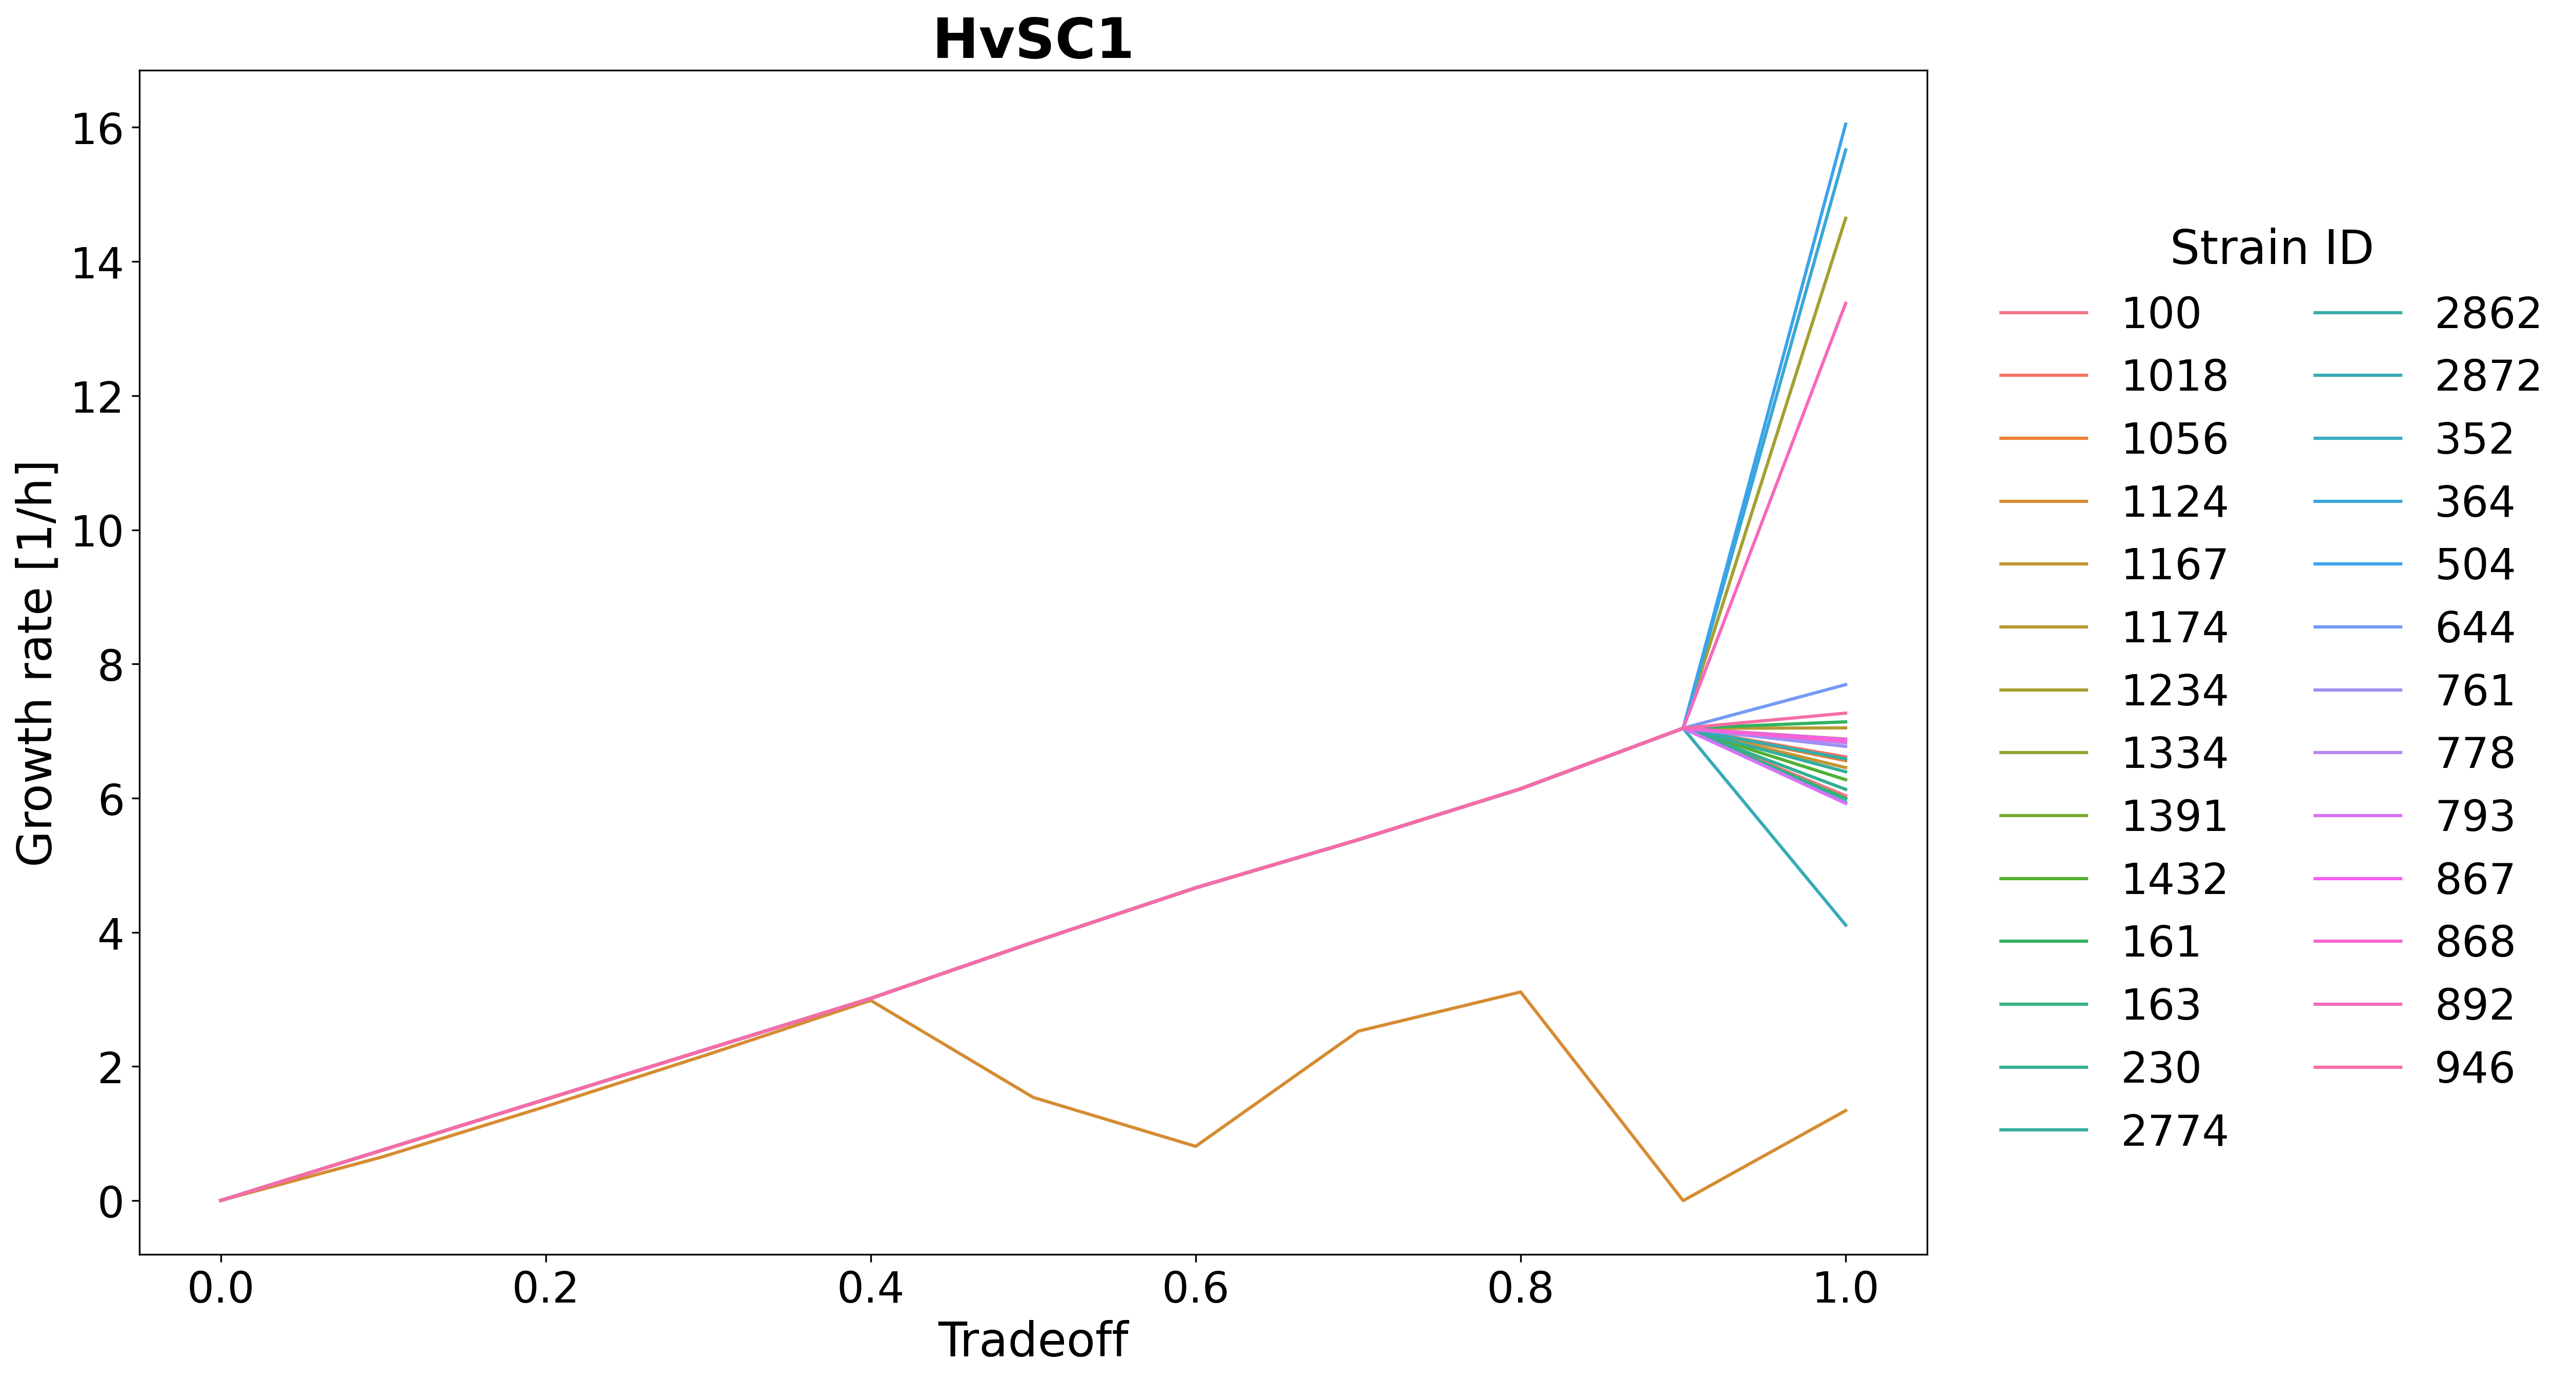
\includegraphics[width=1\linewidth]{fig/HvSC1_individual_growth_tradeoff}
	\caption[Impact of trade-off value $\alpha$ on individual growth rates of HvSC1]{Impact of trade-off value $\alpha$ on individual growth rates of HvSC1. Growth rates of individual community members evaluated at trade-off parameters $\alpha$ between 0.0 and 1.0. Bifurcation of growth rates occurs at $\alpha = 0.96$, strain 1124 diverges at $\alpha = 0.4$. Colour indicates strain ID.}
	\label{fig:hvsc1individualgrowthtradeoff}
\end{figure}

\begin{figure}[H]
	\centering
	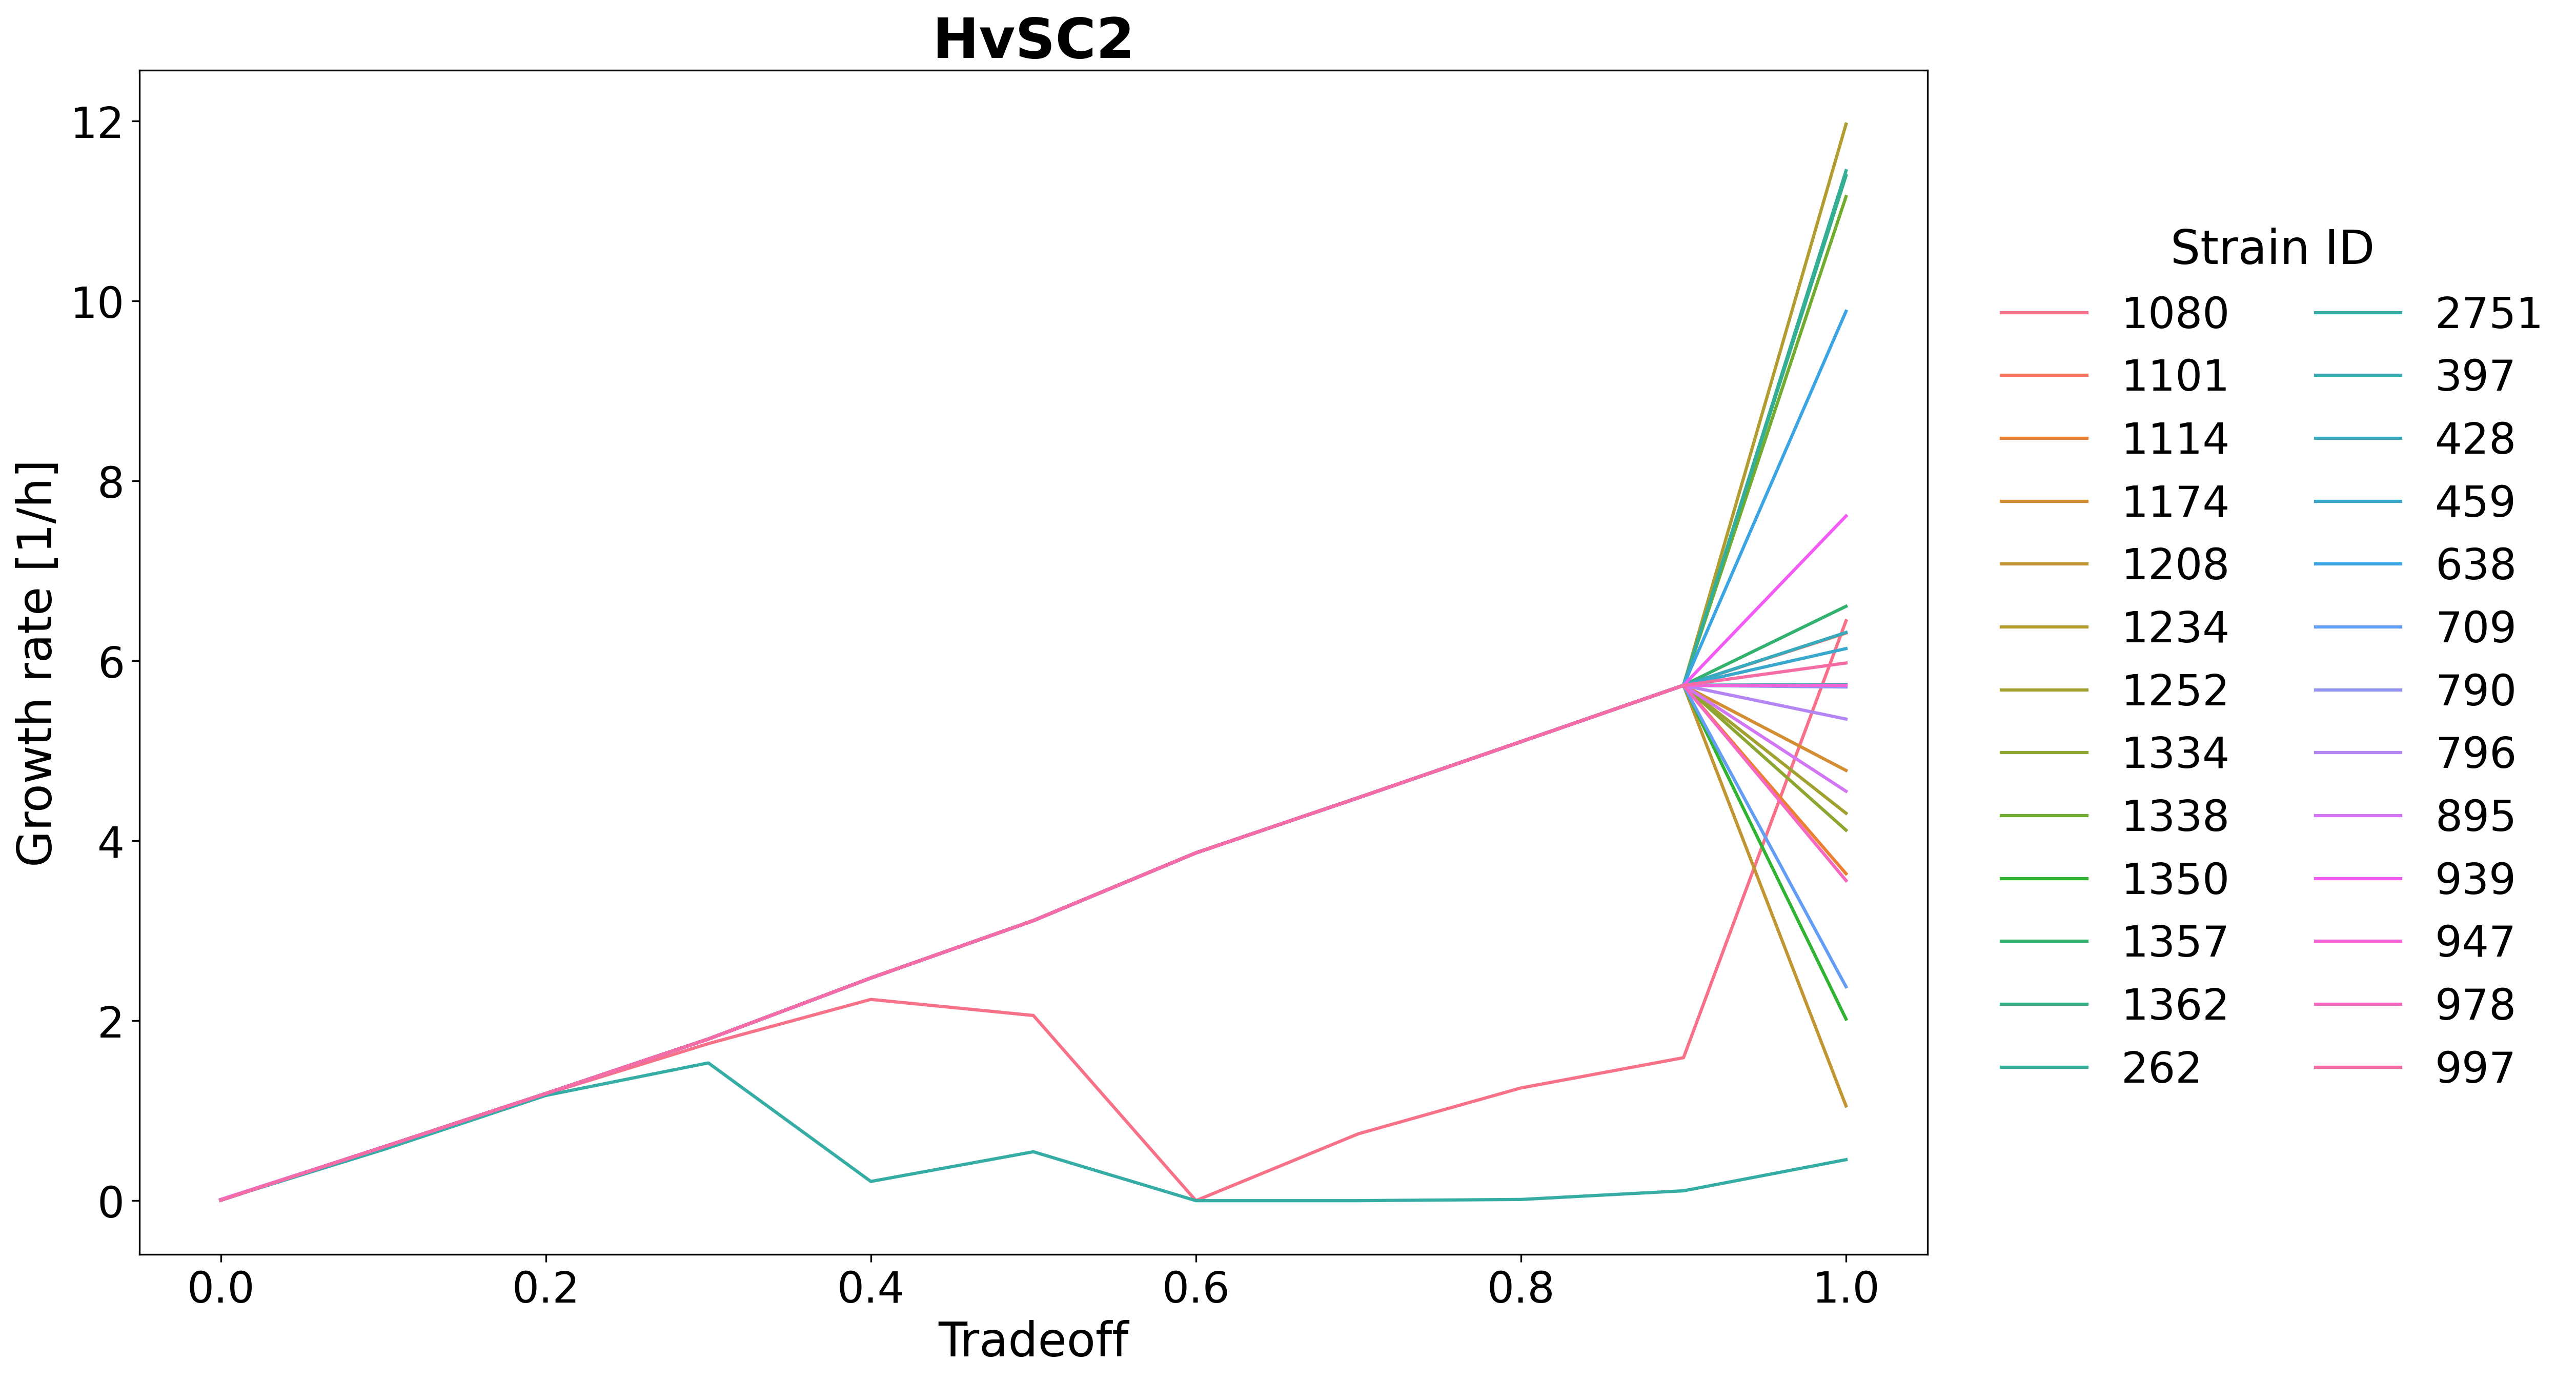
\includegraphics[width=1\linewidth]{fig/HvSC2_individual_growth_tradeoff}
	\caption[Impact of trade-off value $\alpha$ on individual growth rates of HvSC2]{Impact of trade-off value $\alpha$ on individual growth rates of HvSC2. Growth rates of individual community members evaluated at trade-off parameters $\alpha$ between 0.0 and 1.0. Bifurcation of growth rates occurs at $\alpha = 0.96$, with two strains diverging at smaller $\alpha$. Colour indicates strain ID.}
	\label{fig:hvsc2individualgrowthtradeoff}
\end{figure}

\section{Supplementary Tables}

\begin{longtable}{lll}
	\caption{Medium Composition and Exchange Reaction Bounds}
	\label{tab:medium_composition_2}\\
	\toprule
	Compound Name & Exchange Reaction & Upper Uptake Bound \\
	\midrule
	\endfirsthead
	
	\multicolumn{3}{c}%
	{{\tablename\ \thetable{} -- continued from previous page}} \\
	\toprule
	Compound Name & Exchange Reaction & Upper Uptake Bound \\
	\midrule
	\endhead
	
	\midrule
	\multicolumn{3}{r}{{Continued on next page}} \\
	\endfoot
	
	\bottomrule
	\endlastfoot
		(R)-3-Hydroxytetradecanoate & EX\_R\_3httdca\_m & 0.1 \\
		2-Ketogluconate & EX\_2kgnd\_m & 10.0 \\
		4-Aminobutyrate & EX\_4abut\_m & 10.0 \\
		Ammonium & EX\_nh4\_m & 1000.0 \\
		Calcium & EX\_ca2\_m & 1000.0 \\
		Chloride & EX\_cl\_m & 1000.0 \\
		cis-Aconitate & EX\_acon\_C\_m & 0.1 \\
		Citrate & EX\_cit\_m & 10.0 \\
		Cobalt & EX\_cobalt2\_m & 1000.0 \\
		Copper & EX\_cu2\_m & 1000.0 \\
		D-Fructose & EX\_fru\_m & 10.0 \\
		D-Glucose & EX\_glc\_\_D\_m & 10.0 \\
		Diacetylchitobiose & EX\_dachi\_m & 0.1 \\
		Fumarate & EX\_fum\_m & 10.0 \\
		Glycerol & EX\_glyc\_m & 10.0 \\
		Glycine & EX\_gly\_m & 10.0 \\
		Glycyl-L-asparagine & EX\_gly\_asn\_\_L\_m & 10.0 \\
		Glycyl-L-glutamine & EX\_glygln\_m & 10.0 \\
		Iron ($\text{Fe}^{2+}$) & EX\_fe2\_m & 1000.0 \\
		Iron ($\text{Fe}^{3+}$) & EX\_fe3\_m & 1000.0 \\
		L-Alanine & EX\_ala\_\_L\_m & 10.0 \\
		L-Asparagine & EX\_asn\_\_L\_m & 0.1 \\
		L-Aspartate & EX\_asp\_\_L\_m & 10.0 \\
		L-Glutamate & EX\_glu\_\_L\_m & 10.0 \\
		L-Isoleucine & EX\_ile\_\_L\_m & 10.0 \\
		L-Leucine & EX\_leu\_\_L\_m & 10.0 \\
		L-Malate & EX\_mal\_\_L\_m & 10.0 \\
		L-Proline & EX\_pro\_\_L\_m & 0.1 \\
		L-Serine & EX\_ser\_\_L\_m & 10.0 \\
		L-Threonine & EX\_thr\_\_L\_m & 0.1 \\
		L-Tyrosine & EX\_tyr\_\_L\_m & 0.1 \\
		L-Valine & EX\_val\_\_L\_m & 10.0 \\
		Magnesium & EX\_mg2\_m & 1000.0 \\
		Maltose & EX\_malt\_m & 10.0 \\
		Manganese & EX\_mn2\_m & 1000.0 \\
		Molybdate & EX\_mobd\_m & 1000.0 \\
		N-Acetyl-D-glucosamine 1-phosphate & EX\_acgam1p\_m & 0.1 \\
		N-Acetyl-D-mannosamine & EX\_acmana\_m & 0.1 \\
		Nickel & EX\_ni2\_m & 1000.0 \\
		Oxygen & EX\_o2\_m & 1000.0 \\
		Phosphate & EX\_pi\_m & 1000.0 \\
		Potassium & EX\_k\_m & 1000.0 \\
		Proton & EX\_h\_m & 1000.0 \\
		Quinate & EX\_quin\_m & 10.0 \\
		Shikimate & EX\_skm\_m & 0.1 \\
		Sodium & EX\_na1\_m & 1000.0 \\
		Succinate & EX\_succ\_m & 10.0 \\
		Sucrose & EX\_sucr\_m & 0.1 \\
		Sulfate & EX\_so4\_m & 1000.0 \\
		Tyramine & EX\_tym\_m & 10.0 \\
		UDP-N-acetyl-D-glucosamine & EX\_uacgam\_m & 0.1 \\
		Water & EX\_h2o\_m & 1000.0 \\
		Zinc & EX\_zn2\_m & 1000.0 \\
\end{longtable}
	
\begin{longtable}{lllll}
	\caption{Taxonomic classification and Gram stain status of community members}
	\label{tab:syncom_isolates}\\
	\toprule
	Isolate & SynCom & Class & Species & Gram stain \\
	\midrule
	\endfirsthead
	
	\multicolumn{5}{c}%
	{{\tablename\ \thetable{} -- continued from previous page}} \\
	\toprule
	Isolate & SynCom & Class & Species & Gram stain \\
	\midrule
	\endhead
	
	\midrule
	\multicolumn{5}{r}{{Continued on next page}} \\
	\endfoot
	
	\bottomrule
	\endlastfoot
		1174 & Both & Betaproteobacteria & \textit{Hydrogenophaga} sp. BPS33 & negative \\
		1334 & Both & Actinobacteria & \textit{Arthrobacter} sp. FB24 & positive \\
		1234 & Both & Alphaproteobacteria & \textit{Neorhizobium galegae} & negative \\
		892 & HvSC1 & Alphaproteobacteria & \textit{Bosea} sp. F3-2 & negative \\
		2774 & HvSC1 & Chitinophagia & \textit{Paraflavitalea speifideaquilana} & negative \\
		161 & HvSC1 & Betaproteobacteria & \textit{Roseateles chitinivorans} & negative \\
		352 & HvSC1 & Betaproteobacteria & \textit{Polaromonas} sp. JS666 & negative \\
		644 & HvSC1 & Betaproteobacteria & \textit{Acidovorax} sp. A79 & negative \\
		868 & HvSC1 & Betaproteobacteria & \textit{Roseateles} sp. DAIF2 & negative \\
		946 & HvSC1 & Betaproteobacteria & \textit{Variovorax paradoxus} & negative \\
		1018 & HvSC1 & Betaproteobacteria & \textit{Variovorax} sp. WS11 & negative \\
		1056 & HvSC1 & Betaproteobacteria & \textit{Variovorax} sp. KK3 & negative \\
		2862 & HvSC1 & Betaproteobacteria & \textit{Mitsuaria} sp. 7 & negative \\
		100 & HvSC1 & Flavobacteriia & \textit{Flavobacterium soyae} & negative \\
		230 & HvSC1 & Flavobacteriia & \textit{Flavobacterium} sp. MDT1-60 & negative \\
		867 & HvSC1 & Flavobacteriia & \textit{Flavobacterium} sp. RS13.1 & negative \\
		1124 & HvSC1 & Flavobacteriia & \textit{Flavobacterium pectinovorum} & negative \\
		1167 & HvSC1 & Flavobacteriia & \textit{Flavobacterium soyae} & negative \\
		1391 & HvSC1 & Flavobacteriia & \textit{Flavobacterium pectinovorum} & negative \\
		364 & HvSC1 & Gammaproteobacteria & \textit{Stenotrophomonas rhizophila} & negative \\
		2872 & HvSC1 & Actinobacteria & \textit{Nocardioides} sp. B-3 & positive \\
		504 & HvSC1 & Betaproteobacteria & \textit{Pseudoduganella} sp. S-14 & negative \\
		761 & HvSC1 & Betaproteobacteria & \textit{Herbaspirillum hiltneri} & negative \\
		163 & HvSC1 & Gammaproteobacteria & \textit{Pseudomonas} sp. MM213 & negative \\
		793 & HvSC1 & Gammaproteobacteria & \textit{Pseudomonas fluorescens} & negative \\
		778 & HvSC1 & Alphaproteobacteria & \textit{Pararhizobium qamdonense} & negative \\
		1432 & HvSC1 & Alphaproteobacteria & \textit{Shinella zoogloeoides} & negative \\
		709 & HvSC2 & Bacilli & \textit{Bacillus thuringiensis} & positive \\
		2751 & HvSC2 & Bacilli & \textit{Priestia megaterium} & positive \\
		796 & HvSC2 & Alphaproteobacteria & \textit{Caulobacter segnis} & negative \\
		638 & HvSC2 & Actinobacteria & \textit{Cellulomonas} sp. NS3 & positive \\
		1338 & HvSC2 & Chitinophagia & \textit{Chitinophaga filiformis} & negative \\
		428 & HvSC2 & Betaproteobacteria & \textit{Acidovorax} sp. A79 & negative \\
		939 & HvSC2 & Alphaproteobacteria & \textit{Devosia} sp. FJ2-5-3 & negative \\
		1080 & HvSC2 & Alphaproteobacteria & \textit{Devosia rhizoryzae} & negative \\
		262 & HvSC2 & Gammaproteobacteria & \textit{Pseudoxanthomonas} sp. SE1 & negative \\
		1362 & HvSC2 & Gammaproteobacteria & \textit{Lysobacter} sp. S4-A87 & negative \\
		1114 & HvSC2 & Actinobacteria & \textit{Microbacterium} sp. cx-55 & positive \\
		1208 & HvSC2 & Actinobacteria & \textit{Pseudarthrobacter} sp. WHRI 8279 & positive \\
		1350 & HvSC2 & Actinobacteria & \textit{Microbacterium foliorum} & positive \\
		978 & HvSC2 & Actinobacteria & \textit{Nocardioides} sp. W7 & positive \\
		397 & HvSC2 & Gammaproteobacteria & \textit{Pseudomonas chlororaphis} & negative \\
		790 & HvSC2 & Gammaproteobacteria & \textit{Pseudomonas laurylsulfatiphora} & negative \\
		997 & HvSC2 & Gammaproteobacteria & \textit{Pseudomonas} sp. MPB26 & negative \\
		1357 & HvSC2 & Gammaproteobacteria & \textit{Metapseudomonas lalkuanensis} & negative \\
		459 & HvSC2 & Alphaproteobacteria & \textit{Ensifer canadensis} & negative \\
		1101 & HvSC2 & Alphaproteobacteria & \textit{Sinorhizobium} sp. RAC02 & negative \\
		895 & HvSC2 & Alphaproteobacteria & \textit{Sphingomonas hankookensis} & negative \\
		947 & HvSC2 & Alphaproteobacteria & \textit{Sphingomonas} sp. & negative \\
		1252 & HvSC2 & Alphaproteobacteria & \textit{Sphingobium cloacae} & negative \\
\end{longtable}
	